\documentclass[11pt, margin=1in]{article}
\usepackage{amsmath}
\usepackage{amsfonts}
\usepackage[margin=1in]{geometry}
\usepackage{fancyhdr}
\newcommand{\tab}{\par \qquad}
\newenvironment{proof}{ {\it Proof.}}{\hfill\rule{2mm}{2mm}}
\pagestyle{fancy}
\lhead{\textbf{\leftmark}}
\rhead{\textit{Alex Lin, Melissa Yu}}
\cfoot{\thepage}
\renewcommand{\headrulewidth}{0.4pt}
\renewcommand{\footrulewidth}{0.4pt}
\makeatletter

\usepackage{graphicx}
\usepackage{float}
\graphicspath{ {img/} }

%% NOTE: Use \texttt{} for code font.  

\begin{document}

\title{The O-Maze-ing Caml}
\author{Alex Lin and Melissa Yu}
\date{April 27, 2016}
\maketitle

\setlength\parindent{0pt}

% Brief summary here
 
The \textit{O-Maze-ing Caml} is an OCaml-based application that randomly generates mazes and computes the solutions to them.  The program also has graphical capabilities for rendering generated mazes onto the user's screen.  In designing this project, we intentionally employed recursive algorithms to take advantage of OCaml's functional paradigm.  The code can be found at https://github.com/al5250/the-o-maze-ing-caml.  

\section{Overview}

We begin with a high-level description of our project before delving into the specific details within the code files.  Section 2 address the Maze Generation portion of our program, while Section 3 focuses on Maze Solving.  

\subsection{Code Structure}  %% Brief description of main.ml, cell.ml, maze.ml and the code structure (the cell module, the maze functor, etc.)
The code is divided into three files:
\begin{itemize}
\item \texttt{main.ml} - interprets user input and executes the relevant functions of the program  
\item \texttt{cell.ml} - contains the \textsc{Cell} module, which provides implementation for the individual square units that the maze is composed of
\item \texttt{maze.ml} - contains the \textsc{Maze} functor, which provides implementation for maze generation and maze solving based on the \textsc{Cell} module; this file contains the bulk of the project code   
\end{itemize} 


This division was enforced to logically separate the creation of maze modules (\texttt{cell.ml}, \texttt{maze.ml}) from their use (\texttt{main.ml}).  Furthermore, we noted that mazes of different shapes and sizes could be created based on the properties of their cells.  Thus, we packaged the implementation for cells separately from the implementation for mazes; this led us to naturally create a \textsc{Maze} functor that inputed modules of type \textsc{CELL} and outputted modules of type \textsc{MAZE}.
\tab In \textsc{Maze}, we also render the maze and its solution onto a graphical interface as a side effect of the \texttt{generate} and \texttt{solve} functions.  Initially, we considered factoring all of the drawing functions into a separate module, yet we later decided that there was no need for this extra layer of abstraction, as users do not have much of a reason for creating mazes but not viewing them.     

\subsection{Running the Program} %% Explain how to run the program using ./main.byte
To run the program, enter \texttt{./main.byte} into the command line.  You will be prompted with

\begin{flushleft}
\quad \quad \texttt{\# new maze? (y/n): } 
\end{flushleft}

Enter '\texttt{y}' for yes and you will see

\begin{flushleft}
\quad \quad \texttt{\# enter a difficulty (between 1 and 7) to generate maze:}
\end{flushleft}


Entering the number $k$ will prompt the program to randomly generate a maze of size $2^k$ by $2^k$ cells.  

\begin{figure}[H]
\begin{center}
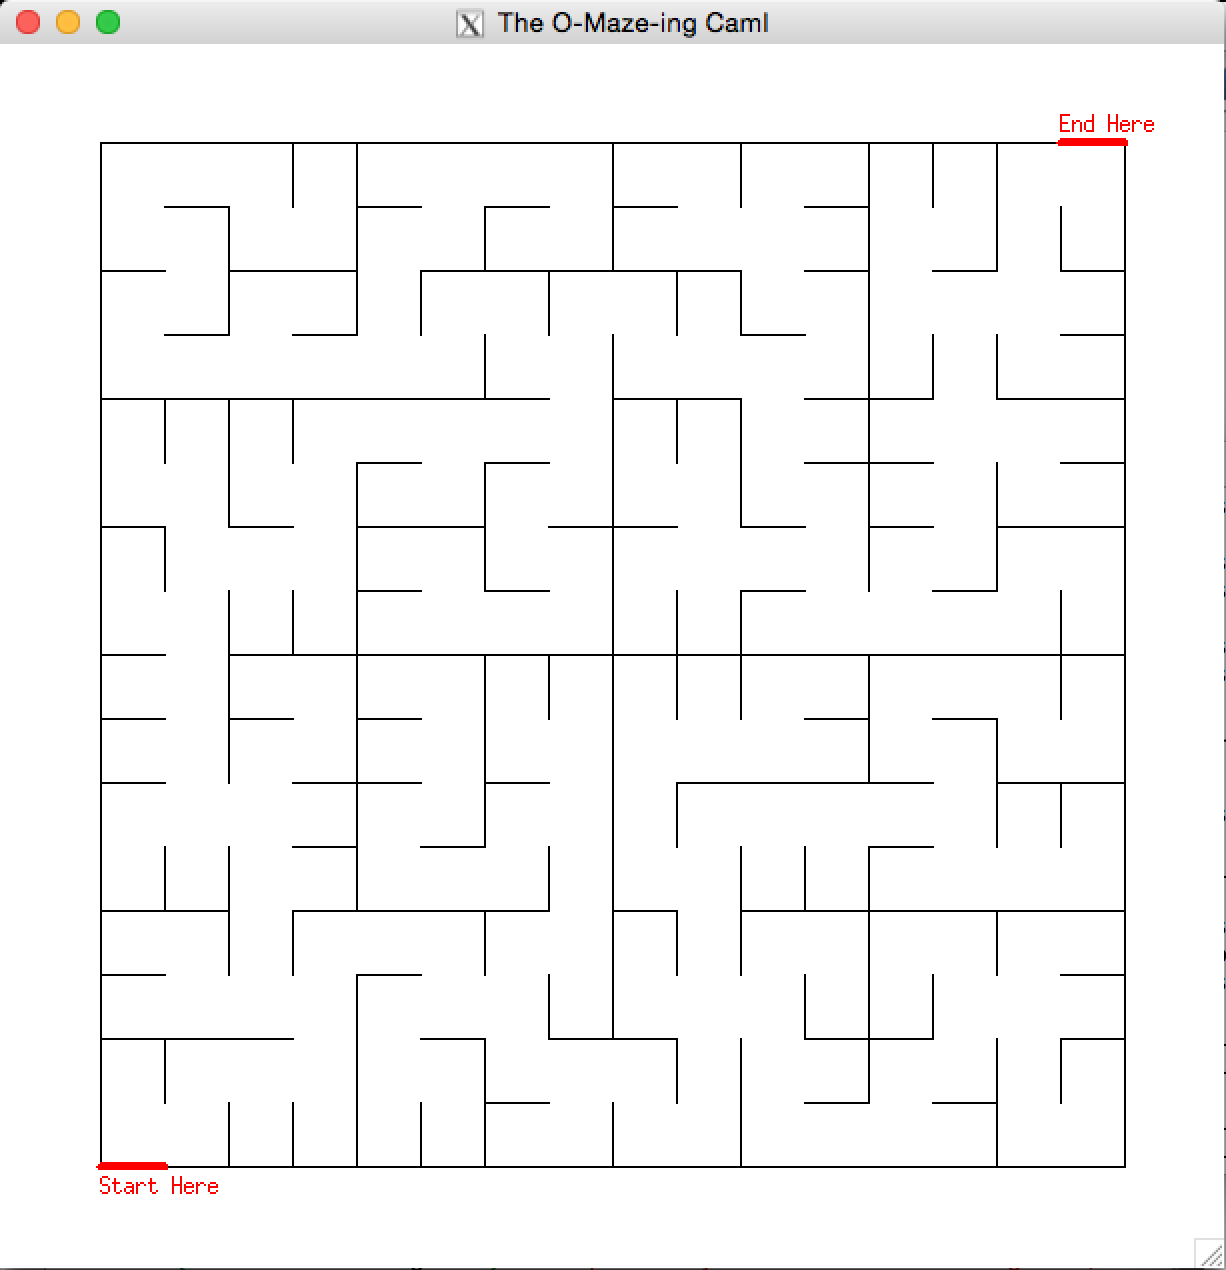
\includegraphics[scale=0.32]{example.jpg}
\caption{An example of a randomly generated $2^4$ x $2^4$ maze.}
\end{center}
\end{figure}

After the maze renders, you will see 

\begin{flushleft}
\quad \quad \texttt{\# see solution? (y/n):}
\end{flushleft}

 
Enter '\texttt{y}' for yes and you will see the solution to your randomly generated maze drawn in red.

\begin{figure}[H]
\begin{center}
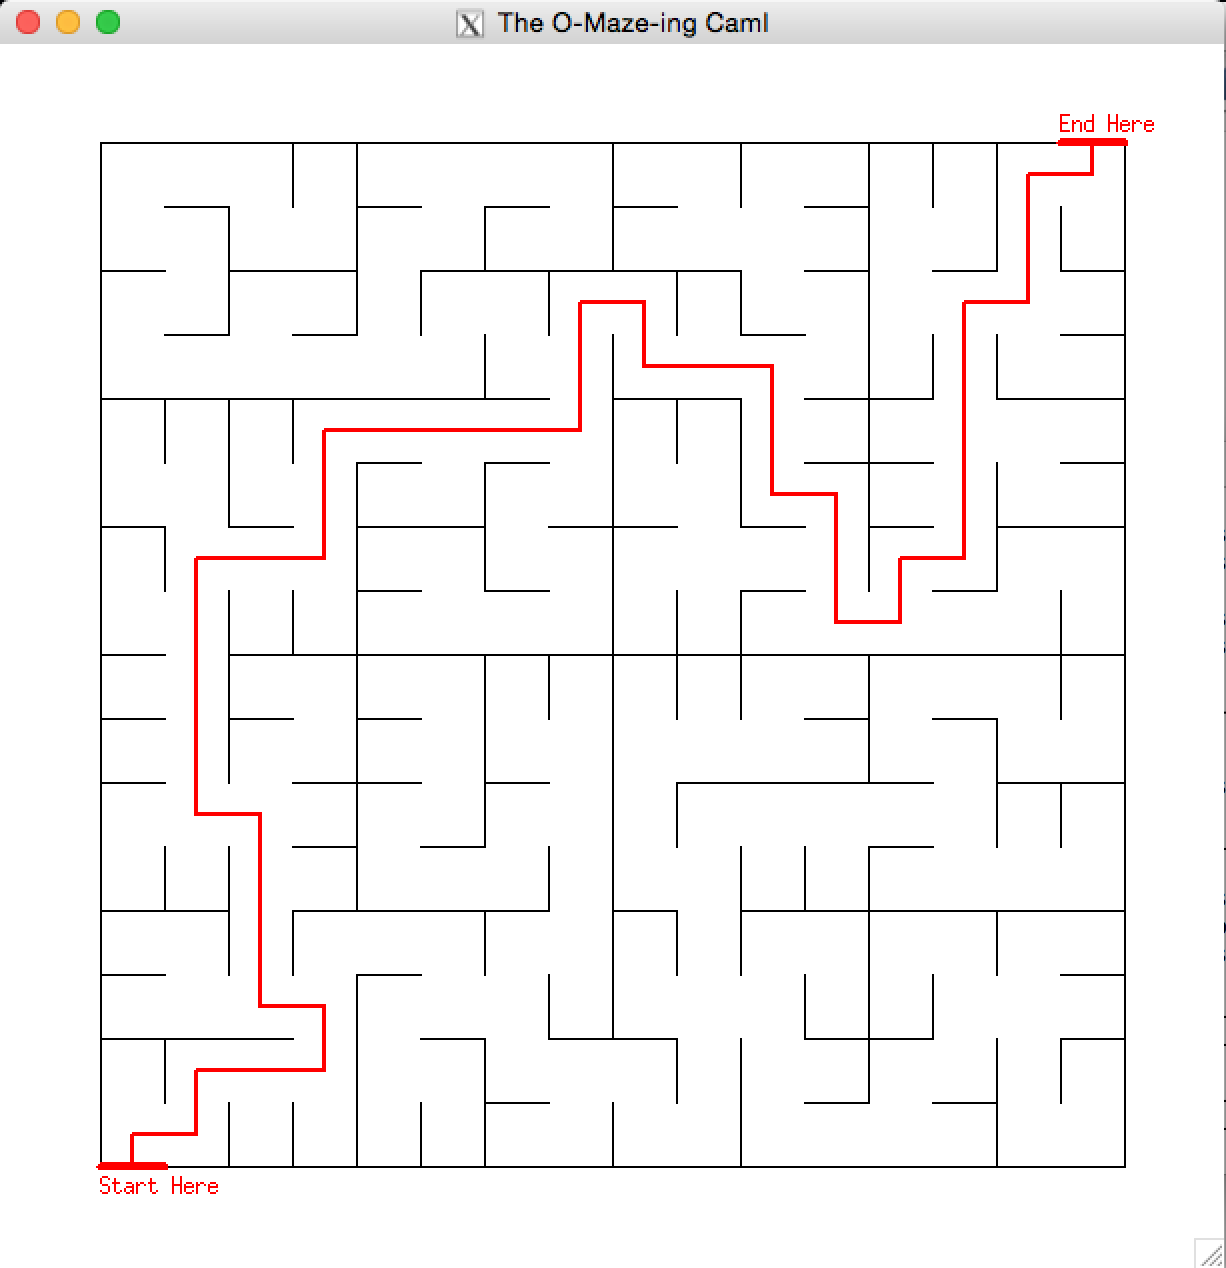
\includegraphics[scale=0.32]{solution.jpg}
\caption{The solution to the above maze.}
\end{center}
\end{figure}


 The program will then loop back to the beginning with 

\begin{flushleft}
\quad \quad \texttt{\# new maze? (y/n): } 
\end{flushleft}


Enter '\texttt{y}' for a new maze and  '\texttt{n}' to quit the program.


    

\section{Maze Generation}

The first of the two major components of our program addresses how to randomly create perfect mazes, given the dimension of the maze. By \emph{perfect maze}, we mean a maze that only has one possible solution.    

\subsection{Recursive-Division Algorithm}  %% Explain theory behind recursive division algorithm, how our algorithm executes it, and the design decisions we made (like the record type cell) 
The recursive division algorithm is the fundamental idea behind how our \texttt{generate} function in \texttt{maze.ml} works.  Although there are many algorithms for maze generation, such as Prim's, Kruskal's, Depth-First Search, etc., we chose recursive division, because it works well with OCaml's functional paradigm.  Mazes are comprised of cells.  Each cell has four sides - top, bottom, left, and right.  Adjacent cells share a side.  Each side can either be \emph{closed} (i.e. there is a wall between the two adjacent cells) or \emph{open} (i.e. there is no wall and one can move freely between the adjacent cells).  
\tab Let's say we want to generate an $n$ by $n$ maze.  The algorithm begins with a single square cell of size $n$ by $n$.   This single cell is then divided into four $\frac{n}{2}$ by $\frac{n}{2}$ cells.  To preserve the maze structure, only one of the four inner cell sides are kept as a wall; the other three are opened.  

\begin{figure}[H]
\begin{center}
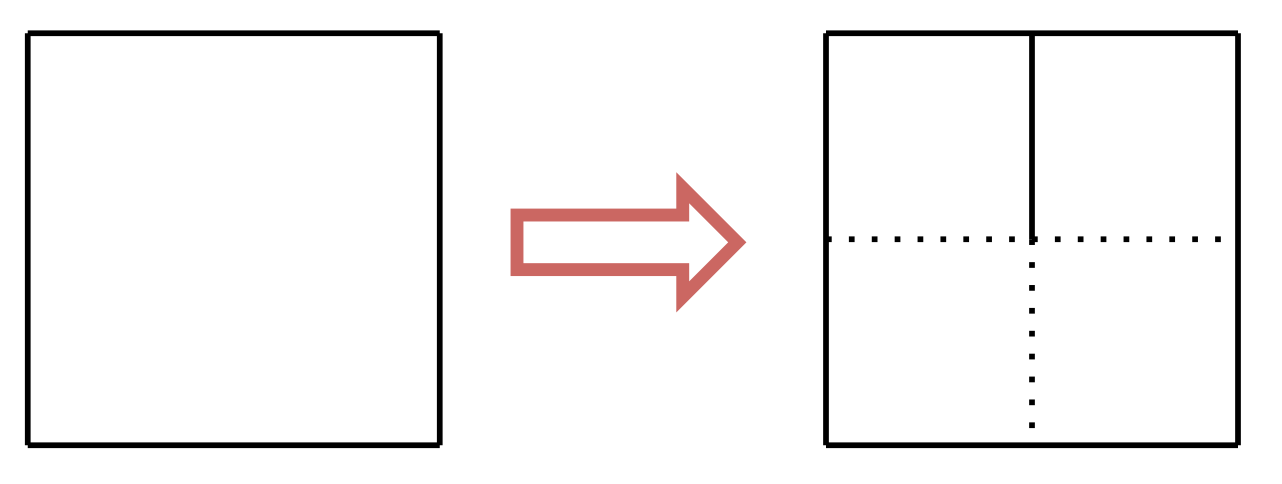
\includegraphics[scale=0.7]{gen1.jpg}
\end{center}
\caption{A cell is divided into four smaller cells.  Only one inner side is kept closed.}
\end{figure}     


Then, the algorithm recursively goes through the same process on each $\frac{n}{2}$ by $\frac{n}{2}$ cell.  During the recursive division process, if an open side of length $m$ is split into two sides of length $\frac{m}{2}$, only one of these sides can be open; the other must be closed.  We do this to preserve the perfect maze invariant; at any point in the algorithm, there can only be one way to get from any cell to any other cell.              

\begin{figure}[H]
\begin{center}
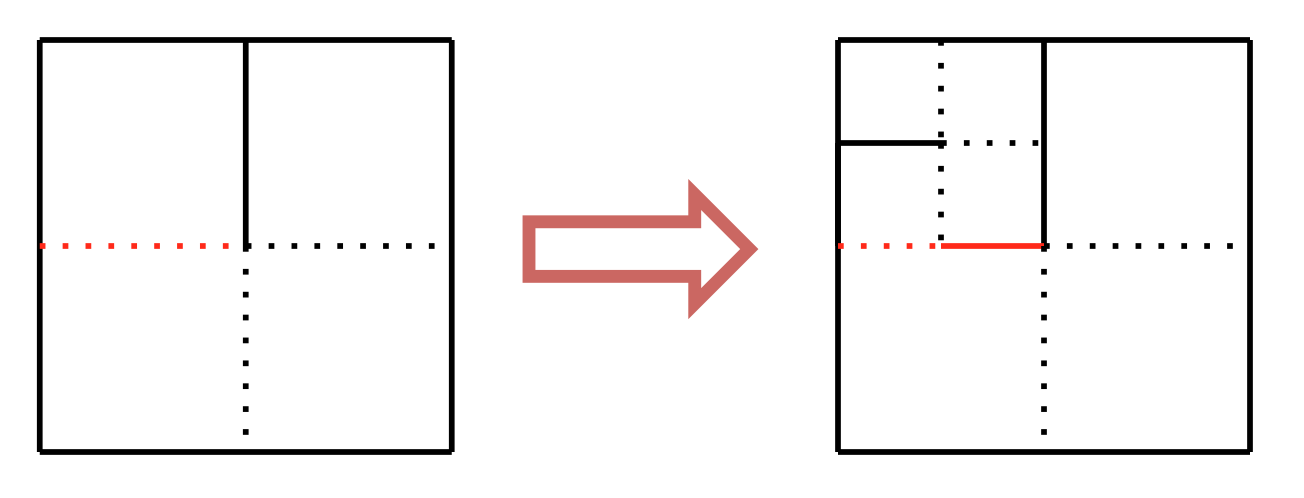
\includegraphics[scale=0.7]{gen2.jpg}
\end{center}
\caption{An open side is divided into 2 smaller sides - one closed and one open (see red).}
\end{figure}

We hit the base case when the length of the cell side is equal to 1.  At this point, we stop dividing and return the resulting perfect maze of $n$ by $n$ cells.  We make two sides on the outer boundary open to have a start point and an end point.    

\tab One advantage of this algorithm is that it is optimally efficient; to produce a maze of $n^2$ cells, it takes $O(n^2)$ time.  Let $T(n)$ be the time it takes to create a $n$ by $n$ maze using recursive division.  The recurrence relation is then
\begin{align*}
T(n) = 4T\left(\frac{n}{2}\right) + c
\end{align*}  
where $c$ is a constant representing the constant work done at each division.  Unraveling the recurrence, we have
\begin{align*}
T(n) &= 4T\left(\frac{n}{2}\right) + c \\
&= 4\left(4T\left(\frac{n}{4}\right) + c\right) + c \\ 
&= 16 T\left(\frac{n}{4}\right) + 5c \\
&= 16 \left(4T\left(\frac{n}{8}\right) + c\right) + 5c \\ 
&= 64 T\left(\frac{n}{8}\right) + 21c \\
& \vdots \\
& = 4^k T\left(\frac{n}{2^k}\right) + (1 + 4 + \ldots + 4^{k-1})c
\end{align*}
We stop when $2^k = n$, or $k = \log_2n$.  Thus, 
\begin{align*}
T(n) = n^2 + (1 + 4 + \ldots + 4^{\log_2n-1}) = n^2 + \frac{4^{\log_2n} - 1}{3} = n^2 + \frac{n^2 - 1}{3} = O(n^2)
\end{align*}
Hence, we have shown that recursive division is optimally fast, because it takes $O(n^2)$ time to produce $n^2$ cell.  Thus, when we made the design decision to implement recursive division over other algorithms such as Prim's, Kruskal's, etc., we did not sacrifice efficiency and simultaneously enabled our program to take advantage of OCaml's functional structure.

\subsection{Design \& Implementation}
 
A natural implementation of the recursive division algorithm is to have \texttt{type cell} be a record that packages relevant variables such as \texttt{pos} (the double indexed position of the lower-left hand corner of the cell in the maze), \texttt{length} (the length of one side of the cell), and booleans for each side of the cell to indicate open (\texttt{true}) or closed (\texttt{false}).  However, if we look at a single side of a cell, we see that it is also the side of another, adjacent cell.  Thus, from the perspective of space efficiency, there is no reason to include this information twice - at least for the process of maze generation.  Therefore, we made the design decision of letting each cell $c$ only keep track of its left and bottom sides (see \texttt{cell.ml}).  The cell above $c$ would keep track of $c$'s top side as its own bottom side and the cell to the right of $c$ would keep track of $c$'s right side as its own left side.  In this fashion, the only sides left untracked are the ones on the outermost boundary of the maze, but these can just all be closed until the algorithm terminates.  Then, two of them will become open for the start and end points of the maze. 

\begin{figure}[H]
\begin{center}
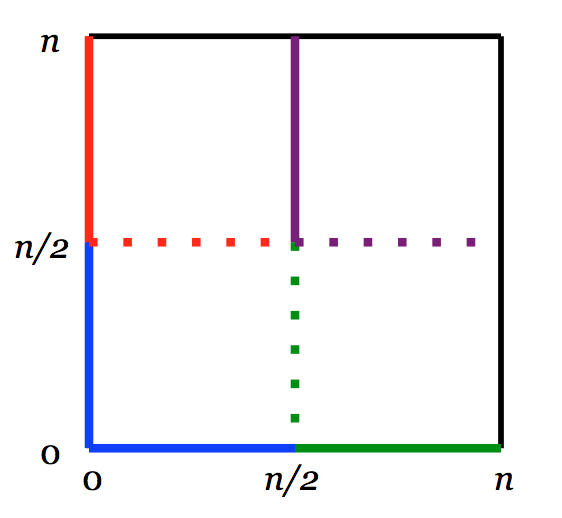
\includegraphics[scale=0.7]{structure.jpg}
\caption{The abstract representation of mazes in our program.  Each color is a different cell.  For example, the green cell is \texttt{\{pos = (n/2, 0); length = n/2; left = true; bottom = false}\}.}
\end{center}
\end{figure}

A more subtle benefit of having each side tracked by only one cell becomes apparent during the process of recursive division.  Let's say we have an open side $s$ that is the right side of cell $c$ and the left side of cell $d$.  During the next step of recursive division, $s$ needs to be split into two smaller sides - $s_1$ and $s_2$.  As explained earlier, exactly one of $s_1$, $s_2$ must be open and the other must be closed, and this will be decided randomly.  The cell-dividing algorithm will be recursively called on $c$ and $d$ separately, but we need to make sure that in each call, the same smaller side (either $s_1$ or $s_2$) is chosen as open and the same smaller side is chosen as closed.  If both $c$ and $d$ kept track of $s$, then enforcing such an invariant would be computationally difficult and inefficient.  On the other hand, by letting only $d$ keep track of $s$ as its left side, we avoid this issue entirely, because $c$ will not process $s$ at all.  This was another factor that played into our decision to let each cell only keep track of its left and bottom sides.    

\tab With the structure of a cell set in place, we can then simply let \texttt{type maze} be a \texttt{cell list}.  Initially, the list will just contain a single cell with side length $n$.  In each iteration of recursive division, the algorithm will process a list of cells with side length $k$ and return a list of cells of side length $\frac{k}{2}$.                   
   
\subsection{Functions Explained} %% Go through each function in generate and explain what it does/how they interact with each other

The main functions which generate a random maze are found in \texttt{maze.ml}:
\begin{itemize}
\item \texttt{initialize} - Creates an empty maze of size $n$, i.e. a single cell at (0, 0) with side $n$, by calling the cell module \texttt{C}'s generate function.
\item \texttt{generate} - Main function used for maze generation. Creates a $n$ by $n$ maze of cells by recursively calling the cell module \texttt{C}'s \texttt{divide} function on the initial cell returned by \texttt{initialize}. Returns the resulting maze as a \texttt{cell list} and draws the maze as a side effect.
\end{itemize}

The functions in \texttt{cell.ml} are recursively called to do the work of actually splitting the cells:
\begin{itemize}
\item \texttt{generate} - Creates a cell with the specified position and dimensions, with the bottom and left walls closed by default. 
\item \texttt{divide} - Divides a single cell into four smaller cells of equal size in two steps. Let's call the original cell $c$. \texttt{divide} does the following: (1) Bisects the bottom and left walls of $c$ to create $c_i$. If the wall being bisected was originally open, \texttt{divide} preserves the perfect maze invariant by calling \texttt{modify}, which chooses one of the two halves of the original wall to remain open (for more detail, see the discussion in 2.1). (2) Randomly sets three of the four inner walls of the divided cell to be open, leaving the remaining one closed.  
\item \texttt{modify} - Randomly chooses one of two input cells to apply the specified function \texttt{f} to. 
\end{itemize}

\subsection{Rendering Graphics} %% Describe how we display the solution to the maze using the Graphics module
Once generated, drawing the maze is straightforward. Using the OCaml \texttt{Graphics} module, which includes functions for creating a new graph, drawing a line between points, and rendering text, we simply initialize an empty graphics window and then iterate through all cells in the maze, drawing each one. The relevant functions are found in \texttt{maze.ml}:

\begin{itemize}
\item \texttt{display\_screen} - Initializes an empty graphics window with a square maze frame and title
\item \texttt{draw\_cell} - Draws a single cell by checking the left and bottom walls of the cell and drawing a line between the current position, $(x, y)$, and $(x, y + dy)$ if the left wall is open, or $(x + dx, y)$ if the bottom wall is open. $dx$ and $dy$ are the scaled lengths of a cell on the display screen. Note that all positions encoded in a cell assume a cell has side length 1 pixel. When rendering a maze, these positions are scaled by a factor determined by the window and maze size.
\item \texttt{draw\_maze} - Iterates through all cells in a maze and calls \texttt{draw\_cell} on each one. Although each iteration of \texttt{draw\_cell} only draws the left and bottom walls of any given cell, iterating through all cells renders the complete picture, since the top and right walls of any given cell are the bottom and left walls of the adjacent cells, and we have already drawn the outermost four walls of the maze in \texttt{display\_screen}. 
\item \texttt{draw} - Main function for drawing unsolved mazes; calls \texttt{display\_screen} and \texttt{draw\_maze}
\end{itemize} 

\section{Maze Solving} 
The second part of our program focuses on the solving of mazes (i.e. how to 

\subsection{Recursive-Backtracking Algorithm} %% Explain theory behind recursive backtracking algorithm, how our algorithm executes it, and the design decisions we made

\subsection{Functions Explained} %% Go through each function in solve and explain what it does/how they interact with each other
To solve the maze, we take advantage of the OCaml \texttt{Array} module, which provides methods for creating n-d matrices and accessing and modifying their elements in place. Two new types, \texttt{array\_cell} and \texttt{array\_maze} are defined in this section to simplify the solution process. Because all cells are the same size after recursive division has concluded, the length parameter becomes redundant, and storing the resulting cells in a matrix allows us to drop the position field as well. Let \texttt{array\_cell} be a four-field record encoding boolean values representing whether each of the four sides of a cell is a wall. Then, the maze is represented by an \texttt{array\_cell array array}. All relevant functions for solving mazes are found in \texttt{maze.ml}:

\begin{itemize}
\item \texttt{to\_matrix} - Converts a \texttt{cell list} to an \texttt{array\_cell array array} representation. Let the current cell being inserted into the array be $c$, with \texttt{c.pos} = $(x, y)$. Then the corresponding array\_cell in the array representation is found at the index $(x, y)$. For each cell popped from \texttt{maze}, we update the left and bottom side values of the corresponding cell in the matrix, as well as the right and top side values of the 2 adjacent neighbors.
\item \texttt{is\_neighbor} - Checks whether 2 given cells communicate (i.e., are both adjacent and directly accessible to each other).
\item \texttt{get\_neighbors} - Returns a list of all communicating cells to the given cell by calling \texttt{is\_neighbor} on the cell's adjacent cells.
\item \texttt{explore} - Extends the path forward one cell in each iteration, until either hitting a dead end, in which case \texttt{backtrack} is called, or reaching the exit cell in the maze, in which case we exit with the final solution path. Let the frontier be the list of unexplored communicating cells adjacent to our current solution path. In each iteration, we pop 1 element off the frontier and check it against the exit conditions. If the conditions are not met, we add the current cell's communicating neighbors to the frontier, rinse, and repeat.
\item \texttt{backtrack} - Backtracks one cell along the current solution path until a new path of exploration is found.   \texttt{backtrack} pops cells off the solution path until reaching a cell that communicates with the next element in frontier, gauged by calling \texttt{is\_neighbor}. At this point, the latest new branch of exploration has been reached, and the function exits back to \texttt{explore}. 
\item \texttt{find\_path} - Finds a solution path for a given \texttt{array\_maze} by initializing \texttt{frontier} and \texttt{path} and calling \texttt{explore}.
\item \texttt{solve} - Main function used for maze solving. Calls \texttt{to\_matrix}, \texttt{find\_path}, and \texttt{draw\_solution} on the given maze, and returns a list of the cells in the solution path in reverse order (i.e., starting with the last cell).
\end{itemize}

\subsection{Rendering Graphics} %% Describe how we display the maze using the Graphics module after generating it
Because drawing the maze is a side-effect of generating one (and thus solve maze will never be called without first having drawing maze), rendering the solution simply requires us to draw the solution path on top of the already rendered graphics. Once again, we use the OCaml \texttt{Graphics} module. All of the functionality is contained in the function \texttt{draw\_solution}, which connects the centers of each cell in the solution path with a line segment.

\end{document}